\documentclass{article} % For LaTeX2e
\usepackage{iclr2025_conference,times}

% Optional math commands from https://github.com/goodfeli/dlbook_notation.
\input{math_commands.tex}

\usepackage{hyperref}
\usepackage{url}
\usepackage{graphicx}
\usepackage{booktabs}
\usepackage{array}

\title{Report Template for MLS}

\newcommand{\fix}{\marginpar{FIX}}
\newcommand{\new}{\marginpar{NEW}}
\newcommand{\warn}[1]{{\color{red}{#1}}}



\begin{document}

\maketitle

% \begin{abstract}
% The abstract paragraph should summarize the whole report in brief. Cover your GLM-ASR kernel implementation (track and key kernels), main optimizations (e.g., kernel fusion, FlashAttention, tile-size tuning), and principal results (speedup over baseline, accuracy preservation). The abstract must be limited to one paragraph.
% \end{abstract}

\section*{Overall Guidelines}

This section contains overall guidelines for using this template to create the report for MLS. Please delete this section in your submitted report.

\begin{description}
\item[Key dates] The deadline for submitting the final report is currently set for 12:00 noon on March 30, 2026, and the deadline for submitting reviews is 12:00 noon on April 13, 2026. Supplementary materials are due at the same time as the report.
\item[Double-blind reviewing] Submissions will be double-blind: reviewers cannot see author names when conducting reviews, and authors cannot see reviewer names. We use OpenReview to host the reports, but all reports and reviews will not be publicly available. Authors can revise their reports as many times as needed up to the submission deadline. Changes to the report will not be allowed while it is under review.
\item[Submission instructions] Please ensure that all authors have an OpenReview profile with the latest information, using their UoE email. Reports must be submitted via the conference submission system at: \url{https://openreview.net/group?id=ed.ac.uk/University_of_Edinburgh/2026/Semester_2/INFR11269}. You should also submit your code as supplementary material, zipped into a single file.
\item[Report length] The main body of the report must not exceed {\bf 8
    pages}. If you have additional material, you may include an appendix.
  The reference list does not count toward the page limit, and unlimited additional pages are allowed
  for the bibliography/references.
  You may include as many appendix pages (after the bibliography) as needed. 
  However, the report must be self-contained, and the assessment will be
  technically and materially based on the main body of the report; markers are
  not required to read the appendix to mark the report.
\item[Report structure] The report should contain exactly seven sections, with fixed section titles as shown in Sections \ref{sec:motivation} to \ref{sec:conclusion}. The subsections and their contents within each section are also fixed. You may add additional optional subsections where indicated.
% \item[Template formatting instructions] All content after Section \ref{sec:conclusion} originates from the original ICLR 2025 {\LaTeX} template. Please refer to their styling guidelines and ignore instructions specifically related to the conference.
\end{description}



\section{Introduction}\label{sec:motivation}

\subsection{Motivation}

In this subsection, you should clearly articulate the motivation for GPU kernel optimization in the context of automatic speech recognition (ASR). Specifically, address the following points:
\begin{itemize}
    \item What is GLM-ASR? Describe the end-to-end pipeline.
    \item Why does GPU kernel optimization matter for inference latency in ASR systems?
    \item What are the computational challenges of implementing custom GPU kernels (e.g., in Triton or cuTile) for a real ASR pipeline?
\end{itemize}

\textbf{GLM-ASR and its pipeline.}
GLM-ASR is a multimodal speech-to-text model that performs end-to-end automatic speech recognition through three sequential components.
Raw audio is first converted into a 128-bin Mel spectrogram and subsampled $2{\times}$ by two 1D convolutional layers.
The resulting sequence is encoded by an \textbf{Audio Encoder}: a 32-layer Transformer with hidden size 1280, 20 attention heads (head dimension 64), intermediate size 5120, LayerNorm normalization, GELU activation, and partial RoPE applied to 50\% of head dimensions.
Its output is then compressed by a \textbf{Multimodal Projector} that concatenates every 4 consecutive frames ($1280{\times}4 = 5120$) and projects through a two-layer MLP ($5120{\to}4096{\to}3584$ with GELU), mapping audio representations into the text embedding space.
Finally, a \textbf{Text Decoder}---a 28-layer Llama-style Transformer with hidden size 3584, Grouped Query Attention (28 Q-heads, 4 KV-heads, head dimension 128), intermediate size 18944, RMSNorm normalization, and SwiGLU gating---autoregressively generates the output token sequence.

\textbf{Why GPU kernel optimization matters.}
ASR inference is latency-critical for real-time applications such as live transcription and voice assistants.
While the Audio Encoder's 32 layers run once per utterance, the Text Decoder's 28 layers execute at every autoregressive decoding step---and since generation cannot be parallelized across output tokens, per-step kernel inefficiencies accumulate linearly with output length.
Without custom GPU kernels, high-level PyTorch operators introduce unnecessary memory allocations, redundant kernel launches, and missed fusion opportunities---all of which inflate end-to-end latency.

\textbf{Challenges of custom kernel implementation.}
Implementing production-quality kernels for GLM-ASR in Triton presents three main challenges.
First, non-power-of-two hidden dimensions (1280, 3584, 18944) require tile-level padding and out-of-bounds masking in every kernel, since Triton requires compile-time constant block sizes that must be powers of two.
Second, the heterogeneous architecture demands structurally distinct kernels: LayerNorm and GELU for the audio path versus RMSNorm and SiLU/SwiGLU for the text path, each with different reduction strategies and memory-access patterns.
Third, GQA in the text decoder (28 Q-heads sharing 4 KV-heads) complicates attention kernel design, and efficient attention must avoid materialising the full $O(\mathrm{seq}^2)$ score matrix---requiring a FlashAttention-style approach that maintains per-block running softmax statistics across tiled K/V blocks while accumulating weighted value sums in registers.

\subsection{System Overview}

This subsection should provide a high-level description of the kernels you
implemented, your key design decisions, and a summary of main findings. This may
include the following:

\begin{itemize}
\item state your track (Triton or cuTile) and list all kernels implemented. 
\item workflow (e.g., Fig.~\ref{fig:asr-pipeline}) showing the path from audio
  input to text output, and where your implemented kernels are used for what
  purpose. 
\item list any optimizations implemented and explain their purpose. 
\item summarize evaluation results: correctness (accuracy) and performance
  (latency). 
\end{itemize}
 

The system architecture can be seen in Fig.~\ref{fig:asr-pipeline}. We implement the system in \textbf{Triton track}.
Table~\ref{tab:kernels} summarises all ten Triton kernels implemented and their roles in the pipeline.

\begin{table}[h!]
\vspace{-1ex}
\centering
\small
\begin{tabular}{lll}
\toprule
\textbf{Kernel} & \textbf{File} & \textbf{Used in} \\
\midrule
\texttt{rmsnorm\_kernel}            & \texttt{layers.py}    & Text Decoder pre-norm \\
\texttt{layernorm\_kernel}          & \texttt{layers.py}    & Audio Encoder pre-norm \\
\texttt{gelu\_kernel}               & \texttt{layers.py}    & Audio Encoder, Projector MLP \\
\texttt{silu\_kernel}               & \texttt{layers.py}    & Text Decoder SwiGLU gate \\
\texttt{linear\_kernel\_tf32}       & \texttt{layers.py}    & All linear projections \\
\texttt{softmax\_kernel}            & \texttt{layers.py}    & Text Decoder output (standalone) \\
\texttt{attention\_scores\_kernel}  & \texttt{attention.py} & $QK^{\top}\!\cdot\!s$ for all heads \\
\texttt{softmax\_inplace\_kernel}   & \texttt{attention.py} & Attention weight normalisation \\
\texttt{attention\_output\_kernel}  & \texttt{attention.py} & $\mathrm{attn}\cdot V$ \\
\texttt{compute\_freqs\_kernel}     & \texttt{rope.py}      & RoPE $\cos$/$\sin$ cache \\
\bottomrule
\end{tabular}
\caption{Implemented Triton kernels and their roles in GLM-ASR.}
\label{tab:kernels}
\vspace{-1.5ex}
\end{table}

We implement three required optimisations:
(1)~\textbf{Tile/block size tuning} for \texttt{linear\_kernel\_tf32} and attention kernels, systematically testing multiple \texttt{BLOCK\_M}/\texttt{BLOCK\_N}/\texttt{BLOCK\_K}, \texttt{num\_warps}, and \texttt{num\_stages} configurations;
(2)~\textbf{Kernel fusion}: \texttt{linear\_gelu\_kernel} (Linear$+$GELU fused) for the Audio Encoder MLP, and \texttt{swiglu\_fused\_kernel} (two Linear projections $+$ SiLU gating in one kernel) for the Text Decoder MLP, eliminating intermediate global-memory round-trips;
(3)~\textbf{FlashAttention-style attention} with online softmax and blockwise $QK^{\top}$/$V$ accumulation, avoiding the $O(\mathrm{seq}^2)$ intermediate score matrix.
Our final implementation achieves \textbf{100.0\%} transcription accuracy and
an end-to-end latency of \textbf{TODO~ms} versus \textbf{TODO~ms} for the Triton baseline
(see Section~\ref{sec:comparison} for full results).

\begin{figure}[h!]
  \begin{center}
\vspace{-0.5ex}    
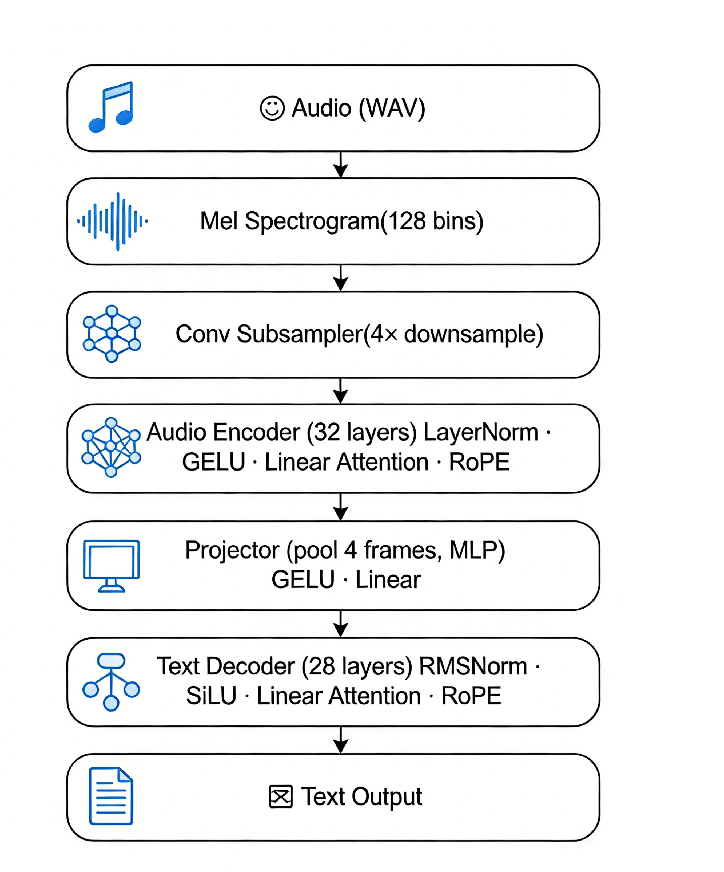
\includegraphics[width=0.4\linewidth]{figure/workflow.png}
\vspace{-0.5ex}    
\end{center}
\caption{GLM-ASR pipeline: Audio $\to$ Mel Spectrogram $\to$ Audio Encoder $\to$
  Projector $\to$ Text Decoder $\to$ Text (highlight the roles of your
  implementation). \warn{Placeholder; replace with your own system architecture.}}
\label{fig:asr-pipeline}
\end{figure}


\section{Implementation}
\label{sec:implementation}

\subsection{Implementation Summary}
Summarize how your implementation is organized across the five phases of the
workflow. For each phase, describe (a) what computation was required in the
corresponding kernels and (b) what the relevant memory-access pattern was, e.g.,
bandwidth-bounded or computation-bounded. 

Our implementation follows the five-phase order recommended in the project guide.
Table~\ref{tab:phases} summarises the computation and memory characteristics of each phase.

\begin{table}[h!]
\vspace{-1ex}
\centering
\small
\resizebox{\linewidth}{!}{%
\begin{tabular}{lm{3.0cm}m{6.5cm}l}
\toprule
\textbf{Phase} & \textbf{Kernels} & \textbf{Computation} & \textbf{Bound} \\
\midrule
1 Element-wise
  & \texttt{silu}, \texttt{gelu}
  & Pointwise $x\sigma(x)$ / tanh-GELU; one read, one write per element
  & Memory \\
2 Reductions
  & \texttt{softmax}, \texttt{softmax\_inplace}, \texttt{rmsnorm}, \texttt{layernorm}
  & One HBM read + write per row. Softmax: $\max \to (x_i - \max) \to \exp \to \sum \to \div$; RMSNorm: $\sqrt{\langle x^2\rangle}\!\to\!wx/\mathrm{rms}$; LayerNorm: $(\mu,\sigma^2)\!\to\!(x{-}\mu)/\sigma{\cdot}w{+}b$
  & Memory \\
3 2D tiled matmul
  & \texttt{linear\_kernel\_tf32}
  & Tiled $A B$ via \texttt{tl.dot} in TF32; accumulator in registers; inner loop over $K$ strips
  & Compute \\
4 Attention
  & \texttt{attention\_scores}, \texttt{attention\_output}
  & $QK^\top{\cdot}s \to \mathrm{softmax\_inplace} \to \mathrm{attn}{\cdot}V$; naive writes $O(T^2)$ score matrix to HBM$^\dagger$
  & Memory$^\dagger$ \\
5 Positional encoding
  & \texttt{compute\_freqs}
  & Precompute $\cos/\sin(p\cdot\theta_i)$ cache; executed once per forward pass
  & Memory \\
\bottomrule
\end{tabular}
}% end resizebox
\caption{Five implementation phases, their kernels, computation, and memory-access characteristics.
$^\dagger$The naive 3-kernel attention is memory-bound due to the $O(T^2)$ score matrix;
the FlashAttention-style replacement (Section~\ref{sec:optimization}) keeps statistics in registers and is compute-bound.}
\label{tab:phases}
\vspace{-1.5ex}
\end{table}


\subsection{Design Choices}

Describe your detailed design specification and justify your choices. This
may include but not limited to: 

\textbf{Block/tile sizes:}
\begin{itemize}
    \item What BLOCK\_SIZE did you choose for element-wise kernels?
    \item What BLOCK\_M / BLOCK\_N / BLOCK\_K did you choose for \texttt{linear\_kernel\_tf32}?
    \item What \texttt{num\_warps} and \texttt{num\_stages} did you use, and why?
\end{itemize}

\textbf{Data layout:}
\begin{itemize}
    \item How did you handle multi-dimensional tensors?
    \item How did you handle GQA head mapping in the Text Decoder?
\end{itemize}




\section{Performance Profiling}\label{sec:profiling}

In this section, you should describe how you profiled and measured the
performance of your implementation.


\subsection{Setup}

Describe your benchmarking setup.


\subsection{End-to-end Evaluation} 


\subsection{Component/Operator-Level Breakdown}



\section{Bottleneck Analysis}\label{sec:bottleneck}

Based on the profiling results from Section~\ref{sec:profiling}, classify each kernel as compute-bound or memory-bound. Use GPU specs (peak TFLOPS, peak bandwidth GB/s) and arithmetic intensity to justify your classification.

\subsection{Compute-Bound vs Memory-Bound Classification}

\subsection{Overall Bottleneck}

Which kernels dominate wall-clock time? Consider non-kernel overheads: launch latency, Python overhead, host-device synchronization, memory allocation vs.\ in-place reuse.

\section{Optimization Attempts}\label{sec:optimization}

Describe at least one optimization (successful or not). Use the \textbf{Hypothesis $\to$ Change $\to$ Result} structure for each optimization.

\subsection{Tile/Block Size Tuning}

\begin{itemize}
    \item \textbf{Hypothesis:} \textit{e.g., ``Larger BLOCK\_M improves occupancy because\ldots''}
    \item Present the configurations tried and explain why the final one was selected.
    \item \textbf{Result:} Which config won? Why? (occupancy, register pressure, shared memory)
\end{itemize}

\subsection{Kernel Fusion (Optional)}

\begin{itemize}
    \item \textbf{Hypothesis:} \textit{e.g., ``Fusing linear+gelu saves one global memory round-trip''}
    \item \textbf{Change:} Before vs.\ after (separate kernels vs.\ fused).
    \item \textbf{Result:} Timing before/after, speedup.
\end{itemize}

If implemented, describe in detail 
\begin{itemize}
    \item which operations did you fuse?
    \item why? 
\end{itemize}


\subsection{FlashAttention-Style Attention (Optional)}

\begin{itemize}
    \item \textbf{Hypothesis:} \textit{e.g., ``What is the memory issue with naive attention?''}
    \item \textbf{Change:} 3-kernel approach $\to$ single fused kernel with online softmax~\citep{dao2023flashattention2fasterattentionbetter}, tiled Q/K/V.
    \item \textbf{Result:} Why is this implementation effective compared to the baseline?
\end{itemize}

If implemented, describe in detail 
\begin{itemize}
    \item how does it differ from the naive 3-kernel approach?
    \item numerical stability (online softmax / log-sum-exp)?
    \item tiling strategy for Q, K, V along the sequence dimension?
\end{itemize}




\subsection{Other Optimizations (Optional)}

\begin{itemize}
    \item Mixed precision (correctness must still pass)
    \item Prefetching / software pipelining (\texttt{num\_stages})
\end{itemize}

\section{Comparison}\label{sec:comparison}

Compare your final implementation (with all optimizations) against the provided example baseline at both component and kernel level.

\subsection{Data Collection}

Describe how you collect and prepare the test dataset(s).
Briefly overview the characteristics of each dataset, especially for those
beyond the provided test cases (if attempted).

\subsection{End-to-End Comparison}

The end-to-end comparison between your final, optimized implementation and
baselines. This may include results about both accuracy and latency. 


\subsection{Per-Operator Comparison}

Like the profiling section, compare per-operator/component performance across
different implementations. 


\subsection{Root Cause Analysis}

For each significant difference, explain the root cause.

\section{Conclusion}\label{sec:conclusion}

Summarize the key findings and contributions of your work. Address the following:
\begin{itemize}
    \item Most impactful optimization and why.
    \item Key lessons: memory-bound vs.\ compute-bound reasoning, why attention is the most challenging kernel to optimize.
    \item Surprising findings from profiling.
    \item What you would try next with more time.
    \item Groupwork contribution (who did what).
\end{itemize}


\clearpage
\bibliography{mybib}
\bibliographystyle{iclr2025_conference}

\appendix
\section{Appendix}
You may include other additional sections here. This does not count toward the
page limit. 
\end{document}
